\documentclass[11pt]{article}
\usepackage{ucs}
\usepackage[utf8x]{inputenc}
\usepackage{changepage}
\usepackage{graphicx}
\usepackage{amsmath}
\usepackage{gensymb}
\usepackage{amssymb}
\usepackage{enumerate}
\usepackage{tabularx}
\usepackage{lipsum}
\usepackage{amsthm}
\usepackage{thmtools}


\usepackage{fontspec} % loaded by polyglossia, but included here for transparency 
\usepackage{polyglossia}

\usepackage{xeCJK}
\setCJKmainfont{SimSun}
\setmainlanguage{russian} 
\setotherlanguage{english}

\newfontfamily\cyrillicfont[Script=Cyrillic]{Times New Roman}
\newfontfamily\cyrillicfontsf[Script=Cyrillic]{Arial}
\newfontfamily\cyrillicfonttt[Script=Cyrillic]{Courier New}

\oddsidemargin 0.0in
\evensidemargin 0.0in
\textwidth 6.27in
\headheight 1.0in
\topmargin 0.0in
\headheight 0.0in
\headsep 0.0in
%\textheight 9.69in
\textheight 9.00in
 
\setlength\parindent{0pt}

\newenvironment{myenv}{\begin{adjustwidth}{0.4in}{0.4in}}{\end{adjustwidth}}
\renewcommand{\abstractname}{Anotācija}
\renewcommand\refname{Atsauces}

%\newenvironment{uzdevums}[1][\unskip]{%
%\vspace{3mm}
%\noindent
%\textbf{#1:}
%\noindent}
%{}

% (4;10;12;17)
% (p1.19;5;15;20)

% http://tex.stackexchange.com/questions/196961/thmtools-declaration-for-theorem-and-proof
\declaretheoremstyle[headfont=\normalfont\bfseries,notefont=\mdseries\bfseries,bodyfont = \normalfont,headpunct={:}]{normalhead}
\declaretheorem[name={Uzdevums}, style=normalhead,numberwithin=section]{problem}

%\def\changemargin#1#2{\list{}{\rightmargin#2\leftmargin#1}\item[]}
\def\changemargin#1#2{\list{}\item[]}
\let\endchangemargin=\endlist 


\newcommand{\subf}[2]{%
  {\small\begin{tabular}[t]{@{}c@{}}
  #1\\#2
  \end{tabular}}%
}



\newcounter{alphnum}
\newenvironment{alphlist}{\begin{list}{(\Alph{alphnum})}{\usecounter{alphnum}\setlength{\leftmargin}{2.5em}} \rm}{\end{list}}

\newenvironment{zhtext}{\fontfamily{MS PGothic}\selectfont}{\par}


\makeatletter
\let\saved@bibitem\@bibitem
\makeatother

\usepackage{bibentry}
%\usepackage{hyperref}

\newenvironment{tulkojums}[1][\unskip]{%
\begin{changemargin}{8mm}{8mm}
\fontsize{9}{11}
\selectfont
\textbf{#1:}
}
{ 
\fontsize{12}{14}
\selectfont
\end{changemargin}
}

\setcounter{section}{1}


\begin{document}

\begin{center}
{\Large \bf Igaunijas 7.-9.kl. uzdevumi ar matemātiskās indukcijas elementiem}
\end{center}

\begin{problem}[EE.PK.1993.9.5]
Rindā izvietotas $n$ ārēji atšķirīgas figūriņas. 
Ir atļauts mainīt vietām jebkuras divas figūriņas, 
starp kurām atrodas tieši viena cita figūriņa. 
Vai ar šādiem pārvietojumiem var visas figūriņas pārlikt
secībā, kura ir pretēja sākotnējai? Pamatot atbildi. 
\end{problem}



\begin{problem}[EE.PK.1994.9.1]
Atrast koeficientu $a_{50}$ šādā identitātē:
$$\left( 1 + x + \ldots + x^{100} \right) \left( 1 + x + \ldots + x^{25} \right)
= 1 + a_1x + \ldots + a_{125}x^{125}.$$
\end{problem}




\begin{problem}[EE.PK.1995.7.3]
Kādā 20-stāvu ēkā lifts sabojāts tādā veidā, ka ar to var 
uzbraukt vai nu 8 stāvus uz augšu, vai arī 11 stāvus uz leju
(ja uz augšu vai uz leju nav tik daudz stāvu, tad attiecīgajā virzienā 
lifts nepārvietojas). 
\begin{enumerate}[(a)]
\item Vai ar liftu var no 20. stāva nobraukt uz pirmo?
\item Uz kuriem stāviem var ar šo liftu aizbraukt no pirmā stāva?
\end{enumerate}
({\em Sk. arī LV.AO.2013.5.2.})
\end{problem}


\begin{problem}[EE.PK.1998.7.TEST.5]
Skaitļi izkārtoti rindās tā, kā parādīts zīmējumā. 
Kāds skaitlis atrodas devītās rindas vidū?
\begin{center}
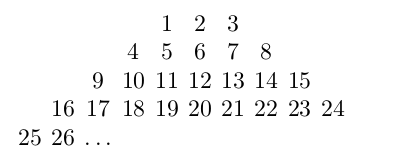
\includegraphics[width=0.4\textwidth]{math-induction-junior-classes/EE-PK-1998-7-TEST-4.png}
\end{center}
\end{problem}

\begin{problem}[EE.PK.2001.8.TEST.5]
Naturālie skaitļi, sākot no $1$, izvietoti 
trijstūrveida tabulā, kuras pirmās četras rindas redzamas zīmējumā. 
Par cik skaitlis, kurš 17.rindā ir pirmais no kreisās, 
ir mazāks par to skaitli, kurš 19.rindā ir pirmais no labās?
\begin{center}
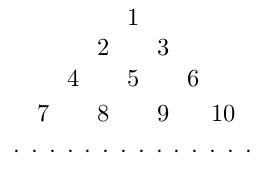
\includegraphics[width=0.25\textwidth]{math-induction-junior-classes/EE-PK-2001-8-TEST-5.png}
\end{center}
\end{problem}



\begin{problem}[EE.PK.2001.8.TEST.5]
Naturālos skaitļus no $1$ līdz $2001$ raksta tabulā, kura 
sastāv no septiņām kolonnām, kā attēlots zīmējumā. 
Ar kādu burtu apzīmēta kolonna, kurā ierakstīs skaitli $2001$?
\begin{center}
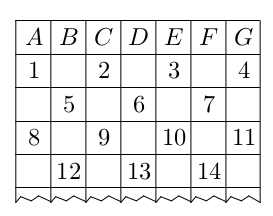
\includegraphics[width=0.25\textwidth]{math-induction-junior-classes/EE-PK-2001-9-TEST-5.png}
\end{center}
\end{problem}

\begin{problem}[EE.PK.2003.9.4]
Zīmējumā attēlota dzelzceļa mezgla shēma. No kreisās puses uz 
labo tam tuvojas $8$ lokomotīves, kuras var virzīties pa 
šo ceļu tikai no kreisās uz labo pusi. 
Parādīt, kā var pārkārtot lokomotīves šajā dzelzceļa mezglā tā, lai 
tās labajā pusē izbrauktu secībā, kas ir pretēja sākotnējai. 
(Katrs ceļa posms šajā mezglā ir pietiekami garš, lai vajadzības 
gadījumā tur novietotos visas lokomotīves.)
\begin{center}
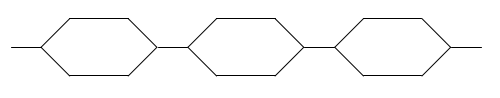
\includegraphics[width=0.4\textwidth]{math-induction-junior-classes/EE-PK-2003-9-4.png}
\end{center}
\end{problem}

\begin{problem}[EE.PK.2004.9.4]
Marija un Juris spēlē sekojošu spēli uz laukuma, 
ko veido $n$ rūtiņu virkne ($n > 2$). 
Katram spēlētājam ir viena figūriņa, abas figūriņas 
spēles sākumā novietotas spēles laukuma abos galos. 
Vienā gājienā spēlētājs pārvieto savu figūriņu par vienu vai 
divām rūtiņām jebkurā virzienā. 
Uzvar tas spēlētājs, kurš novieto savu figūriņu uz tās
rūtiņas, kurā atrodas pretinieka figūriņa. 
Kādām $n$ vērtībām Marijai ir uzvaroša stratēģija; 
pie kādām $n$ vērtībām Jurim ir uzvaroša stratēģija.
\end{problem}

\begin{problem}[EE.PK.2005.9.4]
Doti $2005$ veseli skaitļi. Burvis Merlins spēlē šādu spēli. 
Vienā gājienā viņš izvēlas $7$ skaitļus, un katru izvēlēto 
skaitli (neatkarīgi no citiem izvēlētajiem) palielina par $1$
vai reizina ar $-1$. Pierādīt, ka pēc galīga gājienu skaita 
Merlins var visus $2005$ skaitļus pārvērst par nullēm. 
\end{problem}

\begin{problem}[EE.PK.2006.9.TEST.4]
Atrast izteiksmes vērtību:
$$1 + \frac{100}{2006} - \frac{101}{2006} + \frac{102}{2006} - \frac{103}{2006} + \ldots,$$
ja izteiksme satur $1003$ zīmes ``$+$'' un $1003$ zīmes ``$-$''.
\end{problem}

\begin{problem}[EE.PK.2006.9.4]
Katrs Brīnumzemes iedzīvotājs vai nu vienmēr runā patiesību, vai 
arī vienmēr melo. Reiz visus Brīnumzemes iedzīvotājus sadalīja
pa pāriem un katrs no viņiem pateica par savu pāra kaimiņu 
"Viņš melo" vai arī "Viņš saka patiesību". Vai varēja gadīties, 
ka abi šie apgalvojumi tika izteikti vienādu skaitu reižu, ja 
Brīnumzemē ir {\bf (a)} $2004$ iedzīvotāji?\\
{\bf (b)} $2006$ iedzīvotāji?
\end{problem}


\begin{problem}[EE.PK.2007.7.TEST.6]
Cik dažādos veidos var izveidot skaitli $2007$, sākot ar 
zīmējumā attēloto trijstūrīti, kurā ir cipars $2$ un 
katrā solī pārvietojoties no viena trijstūrīša uz citu, 
kuram ar iepriekšējo ir kopīga mala?
\begin{center}
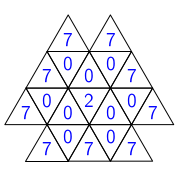
\includegraphics[width=0.2\textwidth]{math-induction-junior-classes/EE-PK-2007-7-TEST-6.png}
\end{center}
\end{problem}


\begin{problem}[EE.PK.2007.8.TEST.6]
Cik dažādos veidos var izveidot skaitli $2007$, ja 
zīmējumā redzamajā figūrā sāk ar aplīti, kurā ir cipars $2$ un 
katrā solī pārvietojas uz citu aplīti, kas pieskaras iepriekšējam? 
\begin{center}
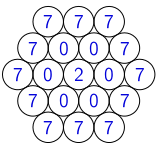
\includegraphics[width=0.2\textwidth]{math-induction-junior-classes/EE-PK-2007-8-TEST-6.png}
\end{center}
\end{problem}


\begin{problem}[EE.PK.2007.9.TEST.6]
Cik dažādos veidos var izveidot skaitli $2007$, sākot ar kvadrātiņu, kurā 
ir skaitlis $2$ un katrā solī pārvietojoties uz citu kvadrātu, kuram ar iepriekšējo ir 
kopīga mala vai kopīga virsotne?
\begin{center}
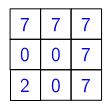
\includegraphics[width=0.15\textwidth]{math-induction-junior-classes/EE-PK-2007-9-TEST-6.png}
\end{center}
\end{problem}

\begin{problem}[EE.PK.2008.9.3]
Rūtiņu laukumā $8 \times 8$ daļa no rūtiņām iekrāsotas 
melnas, bet pārējās \textendash{} baltas. Katrā solī izvēlas
vienu rūtiņu; tad taisnstūrī, kura kreisais augšējais stūris ir 
visa $8 \times 8$ laukuma stūris, bet labais apakšējais stūris 
ir izraudzītā rūtiņa, nomaina visu rūtiņu krāsojumu uz pretējo. 
Vai ar šādiem soļiem no jebkura sākotnējā krāsojuma var sasniegt
stāvokli, kurā visas rūtiņas ir baltas?
\end{problem}


\begin{problem}[EE.PK.2011.7.TEST.10]
Marija salikusi uz galda kaudzīti ar $20$ mandarīniem trijstūra 
piramīdas veidā. Pirmos $10$ mandarīnus viņa liek uz galda tā, 
kā parādīts kreisajā zīmējumā, virs tiem viņa liek slāni no $6$ 
mandarīniem (katrs no kuriem balstās uz trim mandarīniem no zemāk
esošā slāņa), un tā tālāk. 
\begin{center}
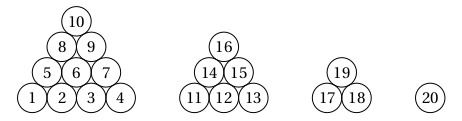
\includegraphics[width=0.6\textwidth]{math-induction-junior-classes/EE-PK-2011-7-TEST-10.png}
\end{center}
Mandarīnus var no kaudzītes paņemt pa vienam. Bet nevar paņemt mandarīnu, kurš
pieskaras tādam mandarīnam, kurš atrodas augstāk. Kāds mazākais skaits mandarīnu 
no kaudzītes jāpaņem, pirms radīsies iespēja dabūt mandarīnu 
{\bf (a)} ar numuru $6$? 
{\bf (b)} ar numuru $4$? 
{\bf (c)} ar numuru $7$?
\end{problem}


\begin{problem}[EE.PK.2011.9.3]
Skaitļiem $x$ un $y$ pieraksts $x \ast y$ apzīmē skaitli 
${\displaystyle \frac{x+y}{xy+4}}$. Atrast izteiksmes vērtību:
$$0 \ast \left(  1 \ast \left( 2 \ast \left( 3 \ast \left(  
4 \ast \left( 5 \ast \left(  6 \ast \left( 
7 \ast \left( 8 \ast 9 \right)
\right) \right) \right)
\right) \right) \right) \right)$$
\end{problem}


\begin{problem}[EE.PK.2017.7.1]
Virknē uzrakstīti $7$ naturāli skaitļi, no kuriem pirmais 
ir $a$ un ir $b$. Katrs nākamais skaitlis šajā virknē vienāds 
ar divu to virknes skaitļu summu, kuri uzrakstīti tieši pirms viņa.\\
{\bf (a)} Atrast pēdējo skaitli šajā virknē, izsakot to ar $a$ un $b$.\\
{\bf (b)} Atrast lielāko iespējamo skaitļa $a$ vērtību, ja zināms, 
ka pēdējais skaitlis virknē ir $2017$.
\end{problem}


\begin{problem}[EE.PK.2017.9.4]
Uz rūtiņu laukuma $8 \times 8$ daļa rūtiņu nokrāsotas baltas, 
bet pārējās melnas. Vienā gājienā var izvēlēties jebkuru 
taisnstūri ar izmēru $2 \times 3$ vai $3 \times 2$, kura 
malas sakrīt ar rūtiņu līnijām, un pārkrāsot visas melnās rūtiņas
baltas un visas baltās rūtiņas melnas. Vai jebkuram sākotnējam krāsojumam 
ar minētajiem gājieniem var iegūt tādu laukumu, kurā 
visas rūtiņas ir melnas?
\end{problem}




\begin{center}
{\Large \bf Lietuvas 5.-8.kl. uzdevumi ar matemātiskās indukcijas elementiem}
\end{center}

\begin{problem}[LT.58.1999.5to7.4]
Karlsonam un Brālītim ir parasta šokolādes tāfelīte ar izmēriem $1999 \times 1999$ kvadrātiņi, 
ko atdala iespiestas rieviņas. Karlsons jebkurā tāfelītes vietā drīkst izlauzt sev
šokolādes gabaliņu ar izmēriem $2 \times 2$ kvadrātiņi, 
bet Brālītis sev - tikai gabaliņu ar izmēriem $1 \times 1$ (visām lauzuma vietām 
jāiet pa rieviņām). Viņi lauž pārmaiņus, pirmais lauž Karlsons. 
Ja kāds no viņiem vairs nevar aprakstītajā veidā izlauzt kvadrātiņu, tad
visa pārpalikusī šokolāde tiek otrajam. Vai var kāds no lauzējiem lauzt tā, 
ka viņam tiktu vairāk nekā puse no visas šokolādes, lai kā arī lauztu otrs. 
\end{problem}


\begin{problem}[LT.58.2003.7to8.1]
Cik ir piecciparu skaitļu, ko var pierakstīt tikai ar cipariem ``$2$'' un ``$5$''
(ne obligāti abiem), turklāt nekādi divi cipari ``$2$'' neatrodas blakus? 
Bet cik ir tādu desmitciparu skaitļu?
\end{problem}

\begin{problem}[LT.58.2005.5to6.2]
Uz četrām vienā plaknē atzīmētām taisnēm atzīmējiet $6$ punktus tā, lai 
uz katras taisnes būtu pa $3$ atzīmētiem punktiem.
\end{problem}

\begin{problem}[LT.58.2005.7to8.1]
Vai uz vienas plaknes piecām taisnēm atzīmēt kopumā $10$ punktus tā, 
ka uz katras no piecām taisnēm būtu pa $4$ atzīmētajiem punktiem? 
\end{problem}

\begin{problem}[LT.58.2008.5to6.3]
Ikreiz, ieraugot skaitli, kurā ir divas pēc kārtas sekojošas nulles, Toms 
satrūkstas. Sestdienās, kad viņiem ir pietiekami laika, Džeris izraksta 
skaitļu virknes un rūpīgi skaita Toma satrūkšanās reizes.
\begin{enumerate}[(a)]
\item Pirmajā sestdienā Džeris izrakstīja visu skaitļu 
virkni no $000$ līdz $999$ un saskaitīja, cik reizes satrūkās Toms. Kādu 
skaitli Džeris ieguva? 
\item Otrajā sestdienā Džeris izrakstīja visu skaitļu virkni 
no $0000$ līdz $9999$ un vēl rūpīgāk saskaitīja, cik reizes satrūkās Toms. 
Kādu skaitli tagad ieguva Džeris?
\item Trešajā sestdienā Džeris jau izrakstīja virknē skaitļus no 
$00000$ līdz $99999$ un vēlreiz rūpīgi saskaitīja, cik reizes satrūkās Toms. 
Cik reizes viņš satrūkās tagad?
\end{enumerate}
\end{problem}

\begin{problem}[LT.58.2011.5to6.3]
Ēzelītis Dainius bija vecs un uzticams zirga Dominika draugs un 
vienmēr mēdza nest Dominikam kādus neredzētus uzdevumus, kurus
no sākuma Dominiks pārāk netiecās risināt. 
Bet, sācis risināt, Dominiks ļoti piktojās, ja viņam neizdevās tos kaut kā pabeigt.
Šodien atnācis, ēzelītis Dainius izvilka no kabatas $16$ salipušus burtu un 
skaitļu pārus: 
$$a1, a2, a3, a4, b1, b2, b3, b4, c1, c2, c3, c4, d1, d2, d3,\text{un}\;d4.$$
un ņēmās mudināt Dominiku uzrakstīt tos salipušos pārus pa vienam katrā tabulas
$4 \times 4$ lodziņā tā, lai katrā tabulas rindiņā un katrā šīs tabulas stabiņā
būtu pa vienai reizei sastopami gan visi četri burti $a,b,c,d$, gan visi 
četri skaitļi $1,2,3,4$.\\
Dominiks ne ļoti tic, ka to var izdarīt, bet ēzelītis Dainius saka, ka to 
vajadzētu varēt kaut vai tādēļ, ka tāda tabula ļoti skaisti izskatītos - 
padomājiet tik: nevienā rindiņā un nevienā stabiņā nekādi burti un skaitļi 
neatkārtojas. Ar ko beigsies šī pāru ierakstīšana?
\end{problem}

\begin{problem}[LT.58.2014.5to6.2]
$9$ elektriskās spuldzītes ir izkārtotas ``kvadrātiskā veidā'' (režģī $3 \times 3$). 
Izglītotais Miškas zina, ka ikvienai spuldzītei ir divi pretēji stāvokļi: 
Stāvoklis "IE" un stāvoklis "IZ". Zaķītis Mikas Paikutis vai cits pilnvarots 
zvēriņš var spiest ar ķepu uz jebkuras spuldzītes. 
Pēc spuldzītes nospiešanas, tās stāvoklis "mainās uz pretējo": Ja līdz nospiešanai 
spuldzīte bija stāvoklī "IE", tad pēc spiešanas tā būs stāvoklī "IZ", un otrādi; 
bez tam, uz pretējo stāvokli pēc nospiešanas pāriet arī visas citas spuldzītes attiecīgajā rindiņā 
un attiecīgajā stabiņā.\\
Sākumā visas $9$ spuldzītes bija stāvoklī "IE". Kāds ir vismazākais spuldzīšu nospiešanu skaits, 
ko jāveic zaķītim Mikam Paikutim, lai visas spuldzītes nonāktu stāvoklī "IZ". 
(Atbilžu varianti: $3$, $4$, $5$, $9$, "to nevar izdarīt".)
\end{problem}


\begin{problem}[LT.58.2014.7to8.5]
Meža vidū stāv liela tāfele, pie kuras rosās $85$ Zaķi, kuri ko prot, ko ne, 
bet viņi visi raksta skaitļus ``gaismas ātrumā''. Kā stāv rakstīts, viņi dzīvo pašā 
Mācītā Meža vidū pie neiedomājama lieluma tāfeles, uz kuras pēc kārtas 
uzrakstīti visi veselie skaitļi no $1$ līdz $2150$.\\
Katrā minūtē cits Zaķis, sākot ar 1. un beidzot ar 85.zaķi pagūst veikt 
ar šiem skaitļiem sekojošu darbību: Ja skaitlis dalās ar $100$, tad to izdala ar $100$, 
bet ja skaitlis ar $100$ nedalās, tad no tāda skaitļa atņem $1$. 
Pēc tam visus agrākos skaitļus nodzēš un to vietā ieraksta iegūtos rezultātus 
(atceramies, ka visus $2150$ skaitļus var nomainīt minūtes laikā - un tā dara katrs zaķis). 
Kāds skaitlis būs lielākais no visiem uz tāfeles uzrakstītajiem, 
kad savas izmaiņas būs beidzis pēdējais, 85.zaķis vārdā Mīkoliņš?
\end{problem}


\newpage

\begin{center}
{\Large \bf Uzdevumi no "Diskrētās matemātikas" mācību grāmatām}
\end{center}

Sākumtekstos veikti labojumi, lai uzdevumi atbilstu olimpiāžu stilam.

\begin{problem}[SusannaEpp.Ch5.P32]
\begin{enumerate}[(a)]
\item $5 \times 5$ kvadrātam izgriezta kaut kāda viena rūtiņa. 
Kurām izgrieztajām rūtiņām atlikušo kvadrātu var sagriezt $L$ formas 
trimino figūriņās? Kuriem nevar? Pamatojiet savu atbildi. 
\item Kādos gadījumos $L$ formas trimino var sagriezt kvadrātus $n \times n$ (Šeit $n > 5$ 
ir patvaļīgs skaitlis, kas nedalās ar $3$). 
\end{enumerate}
\end{problem}

\begin{problem}[SusannaEpp.Ch5.P35]
Pa apli kaut kādā secībā sarakstīti veseli skaitļi no $1$ līdz $30$
katrs tieši vienu reizi. 
\begin{enumerate}[(a)]
\item Vai noteikti atradīsies trīs pēc kārtas uzrakstīti skaitļi, kuru summa ir vismaz $45$?
\item Vai noteikti atradīsies trīs pēc kārtas uzrakstīti skaitļi, kuru summa ir mazāka par $45$?
\end{enumerate}
\end{problem}

\begin{problem}[SusannaEpp.Ch5.P40]
Dots šaha galdiņš ar izmēriem $2n \times 2n$ rūtiņas, kur $n$ ir 
jebkurš naturāls skaitlis. Tā rūtiņas izkrāso pārmaiņus melnas un baltas - tā, lai 
katrām divām rūtiņām ar kopīgu malu būtu atšķirīgs krāsojums. 
Pēc tam no šaha galdiņa izgriež kaut kādas divas rūtiņas - vienu baltu un otru 
melnu. Pierādīt, ka atlikušo figūru varēs sagriezt taisnstūrīšos $1 \times 2$, 
griežot pa rūtiņu līnijām.
\end{problem}

\begin{problem}[Rosen2019.Ch5.P38]
Pieņemsim, ka valstī starp katrām $2$ pilsētām $A$ un $B$ eksistē lidmašīnu satiksme
vienā virzienā (vai nu no $A$ uz $B$, vai arī no $B$ uz $A$). 
Pierādīt, ka eksistē pilsēta, kurā var nokļūt no jebkuras citas pilsētas
vai nu ar tiešu avioreisu vai arī ar vienu pārsēšanos. 
\end{problem}


\begin{problem}[Rosen2019.Ch5.P44]
Racionālus skaitļus formā $p/q$ vēlamies izteikt kā vairāku 
daļu $1/n$ summu, kam skaitītāji ir vienādi ar $1$, bet daļu saucēji 
visi ir atšķirīgi. Piemēram, $5/7 = 1/2 + 1/5 + 1/70$. 
\begin{enumerate}[(a)]
\item Pierādīt, ka jebkuru racionālu skaitli var izteikt kā
$1/n_1 + 1/n_2 + \ldots + 1/n_k$, kur $k \geq 1$ un visi $n_i$ ir dažādi. 
\item Atrast mazāko dažādu saskaitāmo $1/n$ skaitu, lai izteiktu 
$F_{m}/F_{m+1}$, kur $F_m$ ir $m$-tais Fibonači skaitlis. 
Fibonači virkni definē šādi: $F_1 = F_2 = 1$, bet katru nākamo iegūst, saskaitot
divus iepriekšējos virknes locekļus (t.i. virkne ir $1,1,2,3,5,8,13,\ldots$). 
Izsakāmie racionālie skaitļi ir $F_2/F_1 = 1/1$, 
$1/2$, $2/3$, $3/5$, $5/8$, $8/13$, $13/21$ utt.
\end{enumerate}
\end{problem}

\begin{problem}[Rosen2019.Ch5.P49]
Pierādīt, ka $n$ riņķa līnijas sadala plakni $n^2 - n + 2$ apgabalos, 
ja katras divas riņķa līnijas krustojas tieši divos punktos un nekādām 
trim riņķa līnijām nav kopīga punkta.
\end{problem}

\end{document}



